\chapter{Implementation}

In this chapter, the process of implementation will be covered, starting by the architecture and the tools to the results and how everything fits together.

\section{Architecture}
\section{Tools}
\subsection{React JS}

\begin{wrapfigure}[10]{r}{3cm}
	\vspace{-10pt}
	
\includegraphics[width=3cm]{images/chapter3/logo-react-js.png}
	\vspace{-10pt}
	\caption{{\footnotesize React JS framework logo}}
\end{wrapfigure}

React (also known as React.js or ReactJS) is a free and open-source front-end JavaScript library\cite{ReactJavaScriptLibrary} for building user interfaces or UI components. It is maintained by Facebook and a community of individual developers and companies.\cite{ReactMakingFaster} React can be used as a base in the development of single-page or mobile applications. However, React is only concerned with state management and rendering that state to the DOM, so creating React applications usually requires the use of additional libraries for routing, as well as certain client-side functionality.

\subsection{Web3.js}

There are a few different aspects to developing blockchain applications with Ethereum:

\begin{itemize}
\item \textbf{Smart contract development} - writing code that gets deployed to the blockchain with the Solidity programming language.
\item \textbf{Developing websites or clients that interact with the blockchain} - writing code that reads and writes data from the blockchain with smart contracts.
\end{itemize}

\begin{wrapfigure}[9]{r}{3cm}
	\vspace{-10pt}
	
\includegraphics[width=3cm]{images/chapter3/web3.jpeg}
	\vspace{-10pt}
	\caption{{\footnotesize Web3 logo}}
\end{wrapfigure}

Web3.js enables you to fulfill the second responsibility: developing clients that interact with The Etherem Blockchain. It is a collection of libraries that allow you to perform actions like send Ether from one account to another, read and write data from smart contracts, create smart contracts, and so much more.

Web3.js communicates to The Ethereum Blockchain with JSON RPC, which stands for "Remote Procedure Call" protocol. Ethereum is a peer-to-peer network of nodes that stores a copy of all the data and code on the blockchain. Web3.js allows us to make requests to an individual Ethereum node with JSON RPC in order to read and write data to the network\cite{mccubbinIntroWeb3Js}.

\subsection{Ganache}

\begin{wrapfigure}[11]{r}{2.5cm}
	\vspace{-10pt}
	
\includegraphics[width=2.5cm]{images/chapter3/ganache-logo-dark.png}
	\vspace{-10pt}
	\caption{{\footnotesize Ganache Logo}}
\end{wrapfigure}

Ganache is a personal blockchain for rapid Ethereum and Corda distributed application development. You can use Ganache across the entire development cycle; enabling you to develop, deploy, and test your dApps in a safe and deterministic environment.

Ganache comes in two flavors: a UI and CLI. Ganache UI is a desktop application supporting both Ethereum and Corda technology. The command-line tool, ganache-cli (formerly known as the TestRPC), is available for Ethereum development. Prefer using the command-line? This documentation will focus only on the UI flavor of Ganache. Please see the Ganache CLI Readme for command-line documentation.

All versions of Ganache are available for Windows, Mac, and Linux\cite{GanacheOverviewDocumentation}.

\begin{figure}[H]
	\centering
		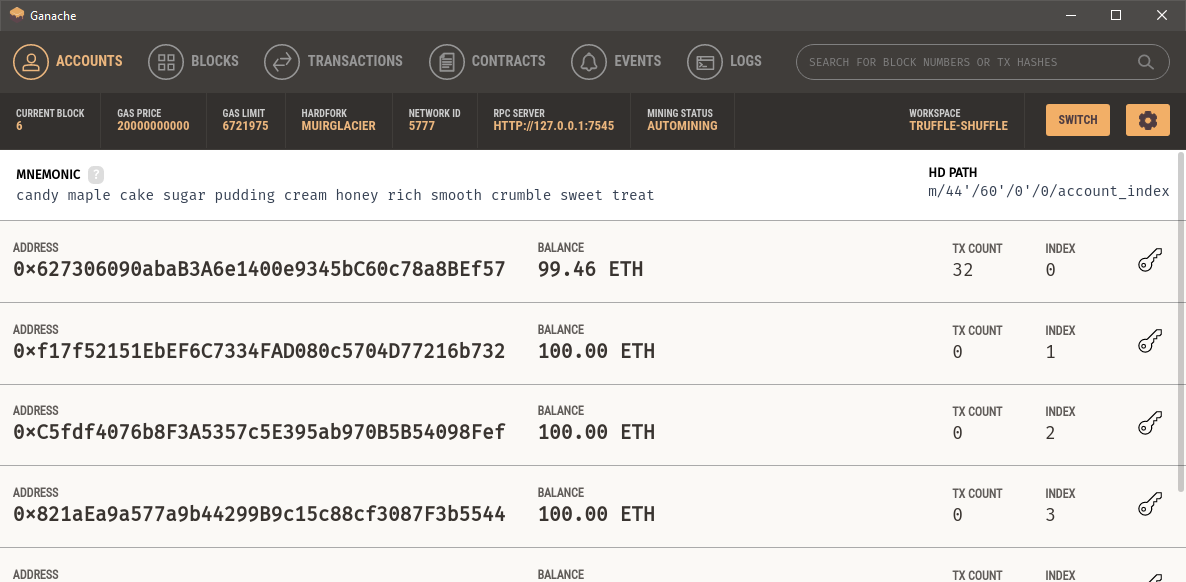
\includegraphics[width=10cm]{images/chapter3/ganache-window.png}
		\caption{{\footnotesize Ganache GUI}}
\end{figure}

\subsection{MetaMask}

\begin{wrapfigure}[10]{r}{2.5cm}
	\vspace{-10pt}
	
\includegraphics[width=2.5cm]{images/chapter3/metamask-logo.png}
	\vspace{-10pt}
	\caption{{\footnotesize MetaMask Logo}}
\end{wrapfigure}

MetaMask is a software cryptocurrency wallet used to interact with the Ethereum blockchain.\cite{schroederCryptoWalletMetaMask2020} It allows users to access their Ethereum wallet through a browser extension or mobile app, which can then be used to interact with decentralized applications.

MetaMask allows users to store and manage account keys, broadcast transactions, send and receive Ethereum-based cryptocurrencies and tokens, and securely connect to decentralized applications through a compatible web browser or the mobile app's built-in browser.[3][4]

The application includes an integrated service for exchanging Ethereum tokens by aggregating several decentralized exchanges (DEXs) to find the best exchange rate. This feature, branded as MetaMask Swaps, charges a service fee of 0.875\% of the transaction amount\cite{schroederCryptoWalletMetaMask2021}.

\begin{figure}[h]
	\centering
		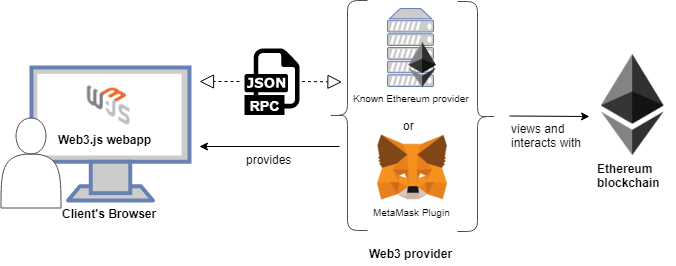
\includegraphics[width=10cm]{images/chapter3/web3-architecture.png}
		\caption{{\footnotesize architecture of a client application interaction with a blockchain network using Web3 and MetaMask}}
\end{figure}

\section{Results}
\subsection{Admin dashboard}
\subsection{End-user (voter) application}
\subsection{Authentication}
\subsection{Smart contract}